\documentclass[a4paper,11pt]{article}

% Шрифты, кодировки, символьные таблицы, переносы
\usepackage{cmap}
\usepackage[T2A]{fontenc}
\usepackage[utf8x]{inputenc}
\usepackage[english, russian]{babel}
% Пакеты американского математического сообщества
\usepackage{amssymb,amsfonts,amsmath,amsthm}  
\usepackage[unicode,hypertexnames=false, colorlinks, urlcolor=magenta, linkcolor=black, pagecolor=black]{hyperref}

% \usepackage[dvipsnames,svgnames]{xcolor}
\usepackage[usenames,dvipsnames]{color} 
\usepackage{graphicx,tabu,hhline,multirow,diagbox}

% \usepackage[utf8]{inputenc}
% commands generated by html2latex


\begin{document}

\section{Цель работы}

Измерение коэффициентов матрицы рассеяния шестиполюсников и установление на основе полученных данных возможных конструктивных вариантов волноводных узлов, находящихся внутри шестиполюсников.

\section{Элементы теории}
\subsection{Основные понятия}

\textbf{Волноводный тракт} состоит из СВЧ-устройств, соединенных определенным образом. Различают \textbf{элементы} и \textbf{узлы} волноводных трактов. Под элементом понимают простейшее устройство, выполняющее одну функцию. Примерами таких устройств могут служить диафрагма, штырь, поршень, сочленение, изгиб или скрутка волновода. Узел состоит из двух или более элементов и представляет собой более широкий класс устройств: трансформатор или фильтр типов волн, аттенюатор, фазовращатель, направленный ответвитель, мостовое соединение, циркулятор и т.д.

Узел связан с трактом с помощью отрезков волновода, которые называются \textbf{плечами} узла. Существуют одноплечие, двухплечие и $N$-плечие узлы. В теории электрических цепей устройства, аналогичные $N$-плечему волноводному узлу, называют $2N$--полюсниками. 
Аналогом простейшего волноводного устройства СВЧ с двумя плечами в теории цепей является четырехполюсник, к входу и выходу которого подсоединены однородные длинные линии. Примерами четырехполюсников являются отрезок волновода, трансформатор с двумя обмотками, фильтры, делители напряжения, усилители. Шестиполюсниками являются трансформатор с двумя вторичными обмотками, волноводный делитель мощности на два канала и т.д.

\subsection{Матричный анализ волноводных узлов}

При наличии в волноводном тракте неоднородных элементов (неоднородностей) анализ распространения электромагнитных волн значительно усложняется. 
Пусть, например, вдоль волновода в прямом направлении (от генератора к нагрузке) распространяется волна только низшего типа (\textbf{падающая волна}). 
Она создает в области неоднородности токи, которые возбуждают в волноводе волны различных типов. 
Суммарное поле падающей волны низшего типа и всех возбуждаемых волн других типов удовлетворяет  граничным условиям на неоднородности.

Среди возбужденных волн отметим \textbf{отраженную волну низшего типа}, распространяющуюся во встречном направлении, \textbf{прошедшую волну} также низшего типа, бегущую в прямом направлении, и группу нераспространяющихся волн высших типов, экспоненциально спадающих при удалении от неоднородности.

Строгое решение соответствующей краевой задачи в принципе позволяет определить как распределение поля вблизи неоднородности, так и связь между амплитудами падающей, отраженной и прошедшей волн.
 Вместе с тем основной интерес для практики представляет отыскание поля волны низшего типа в дальней зоне, т.е. на таком расстоянии от неоднородности, где нераспространяющимися волнами высших типов можно пренебречь.

Эта практическая потребность привела к разработке \textbf{метода эквивалентных схем}, использующего хорошо развитую теорию электрических цепей и длинных линий. 
При таком подходе однородный волновод на низшем типе волны можно заменить эквивалентной ему двухпроводной линией, а неоднородность аппроксимировать сосредоточенными активными и реактивными сопротивлениями, включенными в эту линию.

Для анализа волноводных узлов наряду с методом эквивалентных схем широко применяется \textbf{метод волновых матриц} (рассеяния или передачи). 
Элементами волновых матриц являются непосредственно измеряемые величины -- коэффициенты отражения и передачи, которые характеризуют волновой процесс и устанавливают связь между падающими, отраженными и прошедшими через узел волнами рабочего типа. 
Элементы волновых матриц для данного узла можно рассчитать теоретически при известном решении электродинамической задачи. 
Если же такое решение неизвестно или неизвестно внутреннее устройство узла, элементы волновых матриц находят из эксперимента.

\textbf{Матрицы рассеяния} широко применяются при решении разного рода задач, связанных с согласованием устройств, расчетом погрешностей из-за отражений и т.п. 
При исследовании каскадного соединения нескольких устройств целесообразно использовать \textbf{волновые матрицы передачи}, устанавливающие зависимости амплитуд волн на выходе от амплитуд волн на входе волноводного узла.

\subsection{Волноводная матрица рассеяния}

Рассмотрим трехплечий волноводный узел (шестиполюсник), изображенный на рис. 1. В каждом плече выберем \textbf{плоскость отсчета} (сечение), в котором будем находить отношения амплитуд полей отраженной и падающей волн.

\begin{figure}[h!]
	\centering
	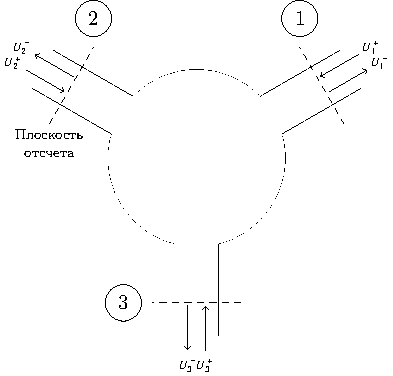
\includegraphics[scale=1.5]{ris/ris1}
	\caption{Схема трехплечего узла (шестиполюсника)}
	\label{fig:figure1}
\end{figure}

Обозначим комплексные амплитуды полей входящих (падающих) в узел волн через $U_m^+$, а амплитуды выходящих (отраженных) волн через $U_k^-$. 
Величины $U_k^-$ зависят от амплитуд и фаз полей волн, входящих во все плечи узла, причем эти зависимости являются линейными в силу линейности уравнений Максвелла (предполагается, что нелинейных элементов в узле нет). 
Связь между амплитудами полей в плечах узла записывается в виде:
\begin{equation}
	\begin{array} { l } { U _ { 1 } ^ { - } = S _ { 11 } U _ { 1 } ^ { + } + S _ { 12 } U _ { 2 } ^ { + } + S _ { 13 } U _ { 3 } ^ { + } } \\ { U _ { 2 } ^ { - } = S _ { 21 } U _ { 1 } ^ { + } + S _ { 22 } U _ { 2 } ^ { + } + S _ { 23 } U _ { 3 } ^ { + } } \\ { U _ { 3 } ^ { - } = S _ { 31 } U _ { 1 } ^ { + } + S _ { 32 } U _ { 2 } ^ { + } + S _ { 33 } U _ { 3 } ^ { + } } \end{array}
\end{equation}
где $S_{km}$ ---  комплексные коэффициенты, характеризующие волноводный узел. 
Их физический смысл очевиден для случая, когда источник включен только в $m$-е плечо ($U_m^+\ne0$), а все остальные плечи нагружены на согласованные нагрузки, и входящие в узел волны в них отсутствуют ($U_i^+=0$, если $i\ne m$). 

В этом случае диагональный элемент $S_{mm}$ представляет собой отношение комплексной амплитуды волны, отраженной от $n$-го входа, к амплитуде волны, поступающей на этот вход:

\begin{equation}
	S _ { m m } = U _ { m } / U _ { m } ^ { + }
\end{equation}
т.е. является коэффициентом отражения волны в $m$-ом плече. Недиагональный элемент $S_{km}$ определяет вклад волны, падающей на $m$-ый вход, в волну, выходящую из $k$-го входа:
\begin{equation}
	S _ { k m } = U _ { k } / U _ { m } ^ { + }
\end{equation}
т.е. является коэффициентом передачи волны из $m$-го плеча в $k$-ое плечо. Систему уравнений (1) удобно записать в матричной форме
\begin{equation}
	\left( \begin{array} { c } { U _ { 1 } ^ { - } } \\ { U _ { 2 } ^ { - } } \\ { U _ { 3 } ^ { - } } \end{array} \right) = \hat { S } \left( \begin{array} { l } { U _ { 1 } ^ { + } } \\ { U _ { 2 } ^ { + } } \\ { U _ { 3 } ^ { + } } \end{array} \right)
\end{equation}
где
\begin{equation}
	\hat { \mathbf { S } } = \left( \begin{array} { c c c } { S _ { 11 } } & { S _ { 12 } } & { S _ { 13 } } \\ { S _ { 21 } } & { S _ { 22 } } & { S _ { 23 } } \\ { S _ { 31 } } & { S _ { 32 } } & { S _ { 33 } } \end{array} \right)
\end{equation}
--- матрица рассеяния, или $S$-матрица (от англ. scattering -- рассеяние).

Из определения элементов матрицы рассеяния (2), (3) следует, что для пассивных узлов, не обладающих свойством усиления мощности, модули коэффициентов передачи и отражения не могут превышать единицы.

\subsection{Свойства волноводных узлов и матриц рассеяния}

\paragraph{Взаимный узел.} Волноводные узлы, в которых отсутствуют элементы с гиротропными свойствами (например, намагниченный феррит), являются взаимными устройствами. Их матрицы рассеяния симметричны относительно главной диагонали

\begin{equation}
	S_{mk}=S_{km}
\end{equation}

Верно и обратное утверждение: если волноводное устройство описывается симметричной матрицей рассеяния, то оно является взаимным.

\paragraph{Волноводное устройство без потерь.} Покажем, что матрица рассеяния волноводного устройства без потерь является унитарной, т.е.

\begin{equation}
	\mathbf { S } ^ { \mathrm { T } } \mathbf { S } ^ { * } = \hat { \mathbf { I } }
\end{equation}

Здесь символы <<$\mathrm { T }$>> и <<$*$>> обозначают операции транспонирования и комплексного сопряжения соответственно. Выражение (6) можно также записать в виде

\begin{equation}
	\sum _ { m = 1 } ^ { N } S _ { l m } ^ { \mathrm { T } } S _ { m k } ^ { * } = \delta _ { l k }
\end{equation}
где $N$ -- число плеч волноводного узла, $\delta_{ik}$ -- индекс Кронекера.

Если в узле отсутствуют источники поля и, кроме того, потерь в узле нет (т.е. элементы узла являются реактивными), то согласно закону сохранения энергии суммарная мощность выходящих волн равна суммарной мощности падающих волн:

\begin{equation}
	\sum _ { m = 1 } ^ { N } \left| U _ { m } ^ { - } \right| ^ { 2 } = \sum _ { m = 1 } ^ { N } \left| U _ { m } ^ { + } \right| ^ { 2 }
\end{equation}

Правую часть выражения (8) перепишем следующим образом:

\begin{equation}
	\sum _ { m = 1 } ^ { N } \left| U _ { m } ^ { + } \right| ^ { 2 } = \sum _ { m = 1 } ^ { N } \left( U _ { m } ^ { + } \right) ^ { * } U _ { m } ^ { + } = \sum _ { m = 1 } ^ { N } \sum _ { k = 1 } ^ { N } \sum _ { l = 1 } ^ { N } \delta _ { m k } \delta _ { m l } \left( U _ { k } ^ { + } \right) ^ { * } U _ { l } ^ { + }
\end{equation}

В свою очередь, левая часть равенства (8) с учетом (1) примет вид: 

\begin{equation}
	\sum _ { m = 1 } ^ { N } \left| U _ { m } ^ { - } \right| ^ { 2 } = \sum _ { m = 1 } ^ { N } \left( U _ { m } ^ { - } \right) ^ { * } U _ { m } ^ { - } = \sum _ { m = 1 } ^ { N } \sum _ { k = 1 } ^ { N } \sum _ { l = 1 } ^ { N } S _ { m k } ^ { * } S _ { m l } \left( U _ { k } ^ { + } \right) ^ { * } U _ { l } ^ { + }
\end{equation}


Тогда из (8) получим

\begin{equation}
	\sum _ { k = 1 } ^ { N } \sum _ { l = 1 } ^ { N } \left\{ \sum _ { m = 1 } ^ { N } \left[ S _ { m l } S _ { m k } ^ { * } - \delta _ { m l } \delta _ { m k } \right] \right\} \left( U _ { k } ^ { + } \right) ^ { * } U _ { l } ^ { + } = 0
\end{equation}

Поскольку $U_k^+, U_l^+$ -- произвольны, выражение в фигурной скобке равно нулю и, следовательно, с учетом

\begin{equation}
	\sum _ { m = 1 } ^ { N } \delta _ { m l } \delta _ { m k } = \delta _ { l k }
\end{equation}
справедливо соотношение
\begin{equation}
	\sum _ { m = 1 } ^ { N } S _ { m l } S _ { m k } ^ { * } = \delta _ { l k }
\end{equation}	

Принимая во внимание, что $S _ { m l } = S _ { l m } ^ { \mathrm { T } }$, приходим к выражению (7). 
Таким образом, доказано, что матрицы рассеяния устройств без потерь унитарны.



Для взаимных волноводных устройств матрица рассеяния является симметричной: $\hat { \mathbf { S } } ^ { \mathrm { T } } = \hat { \mathbf { S } }$. В этом случае из (6) получаем, что для взаимных устройств без потерь

\begin{equation}
	\hat { \mathbf { S } } \hat { \mathbf { S } } ^ { * } = \hat { \mathbf { I } }
\end{equation}

Из формулировки унитарности, представленной в виде (9), следует, что 

\begin{equation}
	\sum _ { m = 1 } ^ { N } S _ { m k } S _ { m k } ^ { * } = \sum _ { m = 1 } ^ { N } \left| S _ { m k } \right| ^ { 2 } = 1
\end{equation}
т.е. сумма квадратов модулей всех матричных элементов любого столбца матрицы рассеяния узла без потерь равна единице. 

Если узел взаимный, то и сумма квадратов модулей всех матричных элементов любой строки также равна единице. 
Кроме того, из (9) следует, что для любой пары столбцов сумма (по строкам) произведений каждого матричного элемента из одного столбца на комплексно сопряженный элемент из той же строки другого столбца равна нулю

\begin{equation}
	\sum _ { m = 1 } ^ { N } S _ { m l } S _ { m k } ^ { * } = 0 , \quad k \neq l
\end{equation}

Очевидно, что для взаимной системы аналогичное соотношение имеет место и для элементов любой пары строк матрицы рассеяния.

\paragraph{Смещение плоскости отсчета.} Предположим, что известна матрица рассеяния при некотором положении плоскости отсчета $z = 0$ в $m$-ом плече узла. При смещении этого сечения на расстояние $l_m$ в направлении распространения падающей волны (по направлению к узлу) новое значение комплексной амплитуды будет

\begin{equation}
	\left( U _ { m } ^ { + } \right) ^ { \prime } = U _ { m } ^ { + } e ^ { - i h _ { m } l _ { m } }
\end{equation}

где $h_m$ -- постоянная распространения волны в $m$-ом плече. Соответственно амплитуда отраженной волны

\begin{equation}
	\left( U _ { m } ^ { - } \right) ^ { \prime } = U _ { m } ^ { - } e ^ { i h _ { m } l _ { m } }
\end{equation}

Если перемещать плоскость отсчета в положительном направлении в первом плече на $l_1$, во втором на $l_2$ и т.д., то волноводный узел будет характеризоваться новой матрицей рассеяния $\hat { \mathbf { S } } ^ { \prime }$, которая связывает новые амплитуды $\left( \mathbf { U } ^ { - } \right) ^ { \prime } = \hat { \mathbf { S } } ^ { \prime } \left( \mathbf { U } ^ { + } \right) ^ { \prime }$. При этом отраженную волну в $m$-ом плече можно записать в виде

\begin{equation}
	(U_m^-)'=S_{m1}'(U_1^+)'+S_{m2}'(U_2^+)'+\ldots+S_{mn}'(U_n^+)'.
\end{equation}

Сравнивая (15) с (1) и учитывая (13), (14), а также произвольность амплитуд, имеем

\begin{equation}
	\begin{array} { l } { S _ { m k } ^ { \prime } = S _ { m k } e ^ { i \left( h _ { m } l _ { m } + h _ { k } l _ { k } \right) } } \\ { S _ { m m } ^ { \prime } = S _ { m m } e ^ { i 2 h _ { m } l _ { m } } } \end{array}
\end{equation}

Таким образом, изменение плоскости отсчета приводит лишь к изменению фазы коэффициентов матрицы рассеяния, не меняя их абсолютного значения. Поскольку выбор плоскостей отсчета произволен, преобразование (16) позволяет в некоторых случаях упростить матричные элементы, сделав их действительными числами.

Перечисленные выше свойства матриц рассеяния используются при расчетах волноводных устройств.

В качестве примера приведем расчет элементов матрицы рассеяния взаимного трехплечего узла без потерь (шестиполюсника), который служит для ответвлении энергии проходящей волны в волноводных трактах.

Рассмотрим так называемый Y-тройник на основе прямоугольного волновода (рис. 2а). 
Плоскости отсчета в каждом из плеч выберем на расстоянии $l=\lambda_B/2$ ($\lambda_B$ --- длина волны в волноводе) от точки 0 пересечения осей соединяемых волноводов. 
Y-тройник обладает пространственной центральной симметрией, вследствие чего все его плечи равноправны по электрическим свойствам, и его эквивалентом является параллельное соединение трех линий (рис. 26). 
Стрелками на рисунках обозначено положительное направление вектора $\mathbf{E}$.

Из симметрии устройства очевидно равенство всех коэффициентов отражения $\Gamma=S_{11}=S_{22}=S_{33}$ и всех коэффициентов передачи $T=S_{12}=S_{13}=S_{23}=\ldots$. Тогда матрица рассеяния Y-тройника имеет вид

\begin{equation}
	\hat { \mathbf { S } } = \left( \begin{array} { c c c } { \Gamma } & { \mathrm { T } } & { \mathrm { T } } \\ { \mathrm { T } } & { \Gamma } & { \mathrm { T } } \\ { \mathrm { T } } & { \mathrm { T } } & { \Gamma } \end{array} \right)
\end{equation}

Определим коэффициенты $\Gamma$ и $\mathrm { T }$. Нагрузкой любого плеча тройника является параллельное соединение двух других линий (рис. 2 в). Импеданс, отвечающий данному соединению, равен 
\begin{equation*}
	Z = \frac { Z _ { \mathrm { H } } Z _ { 0 } } { Z _ { \mathrm { H } } + Z _ { 0 } }
\end{equation*}
($Z_B$ --- волновой импеданс линии), а импеданс $Z_0$ зависит от деталей стыковки плеч тройника и свойств симметричного настроечного элемента, который в принципе может быть помещен в центр тройника (точку 0) без нарушения симметрии системы. 
Для простоты будем считать, что положение настроечного элемента выбрано таким образом, что импеданс $Z_0=iX$, причем $X\to\infty$. В этом случае $Z = Z_H = Z_B/2$ и для коэффициента
отражения в сечении $z=0$ имеем
\begin{equation}
	\Gamma ( 0 ) = \frac { Z - Z _ { \mathrm { B } } } { Z + Z _ { \mathrm { B } } } = - \frac { 1 } { 3 }
\end{equation}

% \begin{figure}[h!]
% 	\centering
% 	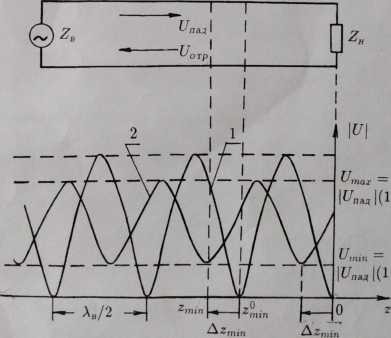
\includegraphics[]{img/2.jpg}
% 	\caption{Y тройник и его эквивалентная схема}
% 	\label{fig:fig2}
% \end{figure}

\begin{figure}[h!]
	\begin{minipage}[t][5cm][t]{0.47\textwidth}
	\center{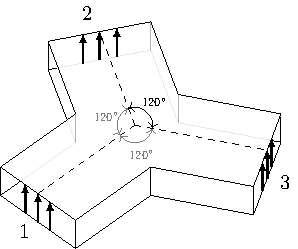
\includegraphics[width=1\linewidth]{ris/ris2a}} \textit{а)} \\
	\end{minipage}
	\hfill
	\begin{minipage}[t][5cm][t]{0.47\textwidth}
	\center{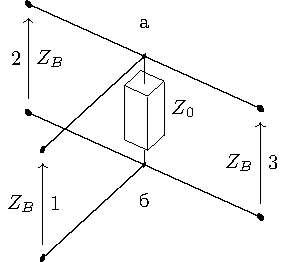
\includegraphics[width=1\linewidth]{ris/ris2b}} \\ \textit{б)}
	\end{minipage}
	\vfill
	\begin{center}
	\begin{minipage}[t][7cm][b]{0.6\textwidth}
	% \hfill
	\center{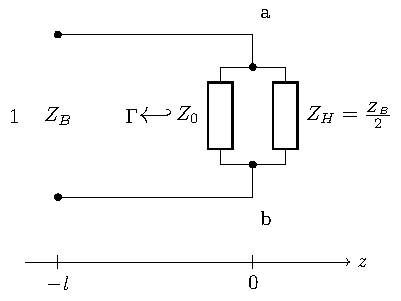
\includegraphics[scale=1.2]{ris/ris2c}} \textit{в)} \\
	% \hfill
	\end{minipage}		
	\end{center}
	\caption{Y тройник и его эквивалентная схема}
	\label{fig:fig2}
\end{figure}


Учтем, что расстояние между плоскостью отсчета $z=-l$, в которой определяется коэффициент отражения, и сечением $z=0$ с импедансом $Z$ (и коэффициентом отражения $\Gamma(0)$) составляет $l=\lambda_B/2$. 
Тогда с помощью формулы пересчета импедансов получим:  $\Gamma = \Gamma(0)$, т.е.  $\Gamma=-\frac13$.

Из условий унитарности (11), (12) следуют соотношения
\begin{equation}
	\begin{array} { c } { | \Gamma | ^ { 2 } + | T | ^ { 2 } + | T | ^ { 2 } = 1 } \\ { \Gamma T ^ { * } + T \Gamma ^ { * } + T T ^ { * } = 0 } \end{array}
\end{equation}
из которых находим: $\mathrm{Re} T = |T| = \frac23$, так что коэффициент передачи $T=\frac23$.

Окончательно, матрица рассеяния волноводного Y-тройника в рассматриваемом случае имеет вид
\begin{equation}
	\hat { \mathbf { S } } = \left( \begin{array} { c c c } { - 1 / 3 } & { 2 / 3 } & { 2 / 3 } \\ { 2 / 3 } & { - 1 / 3 } & { 2 / 3 } \\ { 2 / 3 } & { 2 / 3 } & { - 1 / 3 } \end{array} \right)
\end{equation}
Поскольку $|\Gamma|^2=\frac19$,  $|T|^2=\frac49$, мощность волны, поступающей, например, в первое плечо, делится следующим образом -- 1/9 часть ее отражается, а по 4/9 проходит во второе и третье плечи.

\section{Измерение элементов матрицы рассеяния шестиполюсников}

В работе исследуются пассивные шестиполюсники (трехплечие узлы), т.е. устройства, имеющие три входа (выхода) и не содержащие активных элементов. 
Такое устройство, согласно (1), характеризуется 9 коэффициентами $S_{km}$ ($k,m=1,2,3$). 
Для их определения необходимо провести 9 независимых измерений, на основании которых можно составить 9 линейно независимых уравнений для определения 9 искомых величин. 
Эти измерения можно провести разными способами. 
Желательно, однако, чтобы они были несложными и приводили к простым уравнениям. 
С этой точки зрения удобно производить измерения по следующей схеме.

\subsection{Измерение диагональных элементов}
К плечу 1 (риc. За) через развязывающий аттенюатор (РА) и измерительную линию (ИЛ) подключается генератор электромагнитных  колебаний (Г), а плечи 2 и 3 соединяются согласованными нагрузками (Н). 
При этом в плечах 2 и 3 отраженные от нагрузок волны отсутствуют, т.е. $U _ { 2 } ^ { + } = U _ { 3 } ^ { + } = 0$.


Первое уравнение системы (1) принимает вид $U_1^-=S_{11}U_1^+$, или
\begin{equation}
	S _ { 11 } = U _ { 1 } ^ { - } / U _ { 1 } ^ { + }
\end{equation}
где $U _ { 1 } ^ { - }$ и $U _ { 1 } ^ { + }$ -- комплексные амплитуды отраженной и падающей волн на входе первого плеча шестиполюсника. Отношение этих величин, равное коэффициенту отражения 
\begin{equation}
	\Gamma _ { 11 } = S _ { 11 } = \left| \Gamma _ { 11 } \right| e ^ { i \varphi _ { 11 } }
\end{equation}
можно найти с помощью измерительной линии на основе обычной методики измерения коэффициента стоячей волны и определения положения минимума напряжения (см. Приложение). 
Присоединяя генератор по указанной на рис. За схеме поочередно к плечам 2 и 3, определяют элементы $S_{22}$ и $S_{33}$.

\begin{figure}[h!]
	\centering
	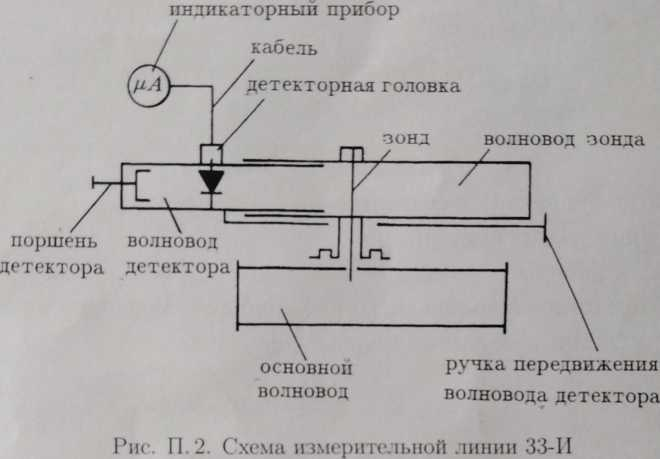
\includegraphics[]{img/3.jpg}
	\caption{Схема измерения элементов $S_{11}$ и $S_{12}$:  Г --- генератор Г4-225, РА  -- развязывающий аттенюатор, ИЛ - измерительная волноводная линия 33-И, СВ - скрутка волновода,  Н -- согласованная нагрузка, КЗ --- короткозамыкатель.}
	\label{fig:fig3}
\end{figure}


% \end{document}
\subsection{Измерение недиагональных элементов}

Рассмотрим другой вариант, отличающийся от предыдущего тем. что плечо 2 короткозамкнуто (рис. 3 6). Теперь лишь $U_3^+=0$, и первые два уравнения системы (1) примут вид
\begin{equation}
	\begin{array} { l } { U _ { 1 } ^ { - } = S _ { 11 } U _ { 1 } ^ { + } + S _ { 12 } U _ { 2 } ^ { + } } \\ { U _ { 2 } ^ { - } = S _ { 21 } U _ { 1 } ^ { + } + S _ { 22 } U _ { 2 } ^ { + } } \end{array}
\end{equation}
Учтем, что в силу граничных условий в точке короткого замыкания амплитуды $U_2^+$ и $U_2^-$ удовлетворяют уравнению
\begin{equation}
	U _ { 2 } ^ { + } = - U _ { 2 } ^ { - }
\end{equation}
Подставляя (20) в (19), находим отношение амплитуд встречных волн в первом плече:
\begin{equation}
	\begin{array} { l } { \Gamma _ { 12 } = \frac { U _ { 1 } ^ { - } } { U _ { 1 } ^ { + } } = S _ { 11 } - S _ { 12 } \frac { U _ { 2 } ^ { - } } { U _ { 1 } ^ { + } } } \\ { \frac { U _ { 2 } ^ { - } } { U _ { 1 } ^ { + } } = \frac { S _ { 21 } } { 1 + S _ { 22 } } } \end{array}
\end{equation}
Подставляя выражение для $U_2^-/U_1^+$ в первое уравнение (21), найдем коэффициент отражения $\Gamma_{12}$ на входе первого плеча шестиполюсника, включенного по схеме, изображенной на рис. 3б:
\begin{equation}
	\Gamma _ { 12 } = S _ { 11 } - \frac { S _ { 12 } S _ { 21 } } { 1 + S _ { 22 } }
\end{equation}
Тогда для произведения недиагональных элементов матрицы рассеяния имеем
\begin{equation}
	S _ { 12 } S _ { 21 } = \left( 1 + S _ { 22 } \right) \left( S _ { 11 } - \Gamma _ { 12 } \right)
\end{equation}
Поскольку диагональные элементы $S_{mm}$ известны (из предыдущих экспериментов), а коэффициент отражения $\Gamma_{12}=|\Gamma_{12}|е^{i\phi_{12}}$ можно найти с помощью измерительной линии, то этот эксперимент дает возможность определить произведение $S_{12}S_{21}$.
При такой методике измерения невозможно определить отдельно элементы $S_{12}$ и $S_{21}$, однако, если шестиполюсник не содержит невзаимных элементов, то, согласно (5), $S_{12} = S_{21}$ и $S_{12}S_{21}=S_{12}^2$. 
Поэтому (возможно ошибка в знаке)
\begin{gather}
	S _ { 12 } = \sqrt { S _ { 12 } S _ { 21 } } = \nonumber \\= \left\{ \left[ \operatorname { Re } \left( S _ { 12 } S _ { 21 } \right) \right] ^ { 2 } + \left[ \operatorname { Im } \left( S _ { 12 } S _ { 21 } \right) \right] ^ { 2 } \right\} ^ { 1 / 4 } \exp \left[ \frac { 1 } { 2 } \operatorname { arctg } \frac { \operatorname { Im } \left( S _ { 12 } S _ { 21 } \right) } { \operatorname { Re } \left( S _ { 12 } S _ { 21 } \right) } \right]
\end{gather}

Аналогично, закорачивая плечо 3 и присоединяя согласованную нагрузку к плечу 2, найдем 
\begin{equation}
	S _ { 13 } S _ { 31 } = S _ { 13 } ^ { 2 } = \left( 1 + S _ { 33 } \right) \left( S _ { 11 } - \Gamma _ { 13 } \right)
\end{equation}
где  $\Gamma _ { 13 } = \left| \Gamma _ { 13 } \right| e ^ { i \varphi _ { 13 } }$ -- коэффициент отражения на входе первого плеча в данной схеме включения шестиполюсника.

Для определения произведения $S_{23}S_{32}=S_{23}^2$ генератор следует
присоединить к плечу 2, нагрузку -- к плечу 1, а плечо 3 закоротить.
Тогда
\begin{equation}
	S _ { 23 } ^ { 2 } = \left( 1 + S _ { 33 } \right) \left( S _ { 22 } - \Gamma _ { 23 } \right)
\end{equation}
где $\Gamma _ { 23 } = \left| \Gamma _ { 23 } \right| e ^ { i p _ { 23 } }$ коэффициент отражения на входе плеча 2.

Таким образом, шесть описанных выше экспериментов дают возможность полностью определить все параметры  шестиполюсника.
Если шестиполюсник содержит невзаимные элементы, для отыскания его параметров следует производить 9 независимых экспериментов, причем необходимо также иметь возможность измерения величины сигнала, прошедшего в данное плечо.

\section{Задания и порядок выполнения работы}

\begin{enumerate}
	\item Ознакомиться с устройством и работой генератора Г4-225 и измерительной волноводной линией 33-И. Включить и подготовить к работе генератор. Рекомендуемое значение несущей частоты генератора -- 8,5 ГГц. Необходимо учесть, что аттенюатор в блоке генератора является развязкой между генератором и нагрузкой, для удобства работы обычно используется значение затухания $-3\ldots-6$ дБ.
	\item Закоротить с помощью короткозамыкателя (КЗ) измерительную линию, на конце которой должна находиться скрутка волновода. Резонатор измерительной линии настроить на максимум показаний индикатора. Далее зонд измерительной линии установить в ближайший к концу линии узел стоячей волны. Координата узла $z^0_{min}$ принимается за условный конец линии. Измерить длину волны в волноводе $\lambda_B$.
	\item Присоединить к скрутке волновода на конце измерительной линии каждую из двух используемых при выполнении работы согласованных нагрузок. Определить коэффициенты отражения от них $\Gamma_{H1,2}$ (см. приложение). Значения  $\Gamma_{H1,2}$ определяют точность расчетов элементов матриц рассеяния шестиполюсников по формулам (18), (23)-(25).
	\item Измерить параметры шестиполюсников в предположении, что они являются взаимными. 

	Для каждого из предложенных шестиполюсников осуществить 6 описанных выше экспериментов. По данным измерений заполнить таблицу.

	Элементы матрицы рассеяния $S_{km}$ рассчитываются по данным таблицы и формулам (18), (23)-(25). Вначале следует рассчитать диагональные элементы, а затем -- недиагональные. Результаты записываются в виде $S _ { k m } = \left| S _ { k m } \right| e ^ { i \varphi _ { k m } }$.
	\item Установить возможные конструктивные варианты волноводных узлов, образующих исследуемые шестиполюсники.
\end{enumerate}

% Образец заполнения экспериментальных данных при выполнении работы:

% $$
% z_{\min}^0=\ldots, \lambda_B=\ldots
% $$

% \begin{tabular}{|c|c|c|c|c|c|c|c|c|c|c|} 
% \hline
% \multirow{2}{*}{\vspace{-1em}№} & $S_{km}$ &  \multicolumn{3}{c|}{№ входа}  & \multicolumn{2}{c|}{1}                         & \multicolumn{2}{c|}{2}                         & \multicolumn{2}{c|}{3}                         \\ \hhline{|~|~|-|-|-|-|-|-|-|-|-|}
%   &          & 1 & 2 & 3 & \diagbox{$I_{\max}$ }{$I_{\min}$ } & $z_{\min}$ & \diagbox{$I_{\max}$ }{$I_{\min}$ } & $z_{\min}$ & \diagbox{$I_{\max}$ }{$I_{\min}$ } & $z_{\min}$ \\ \hline
% \end{tabular}

\section{Контрольные вопросы}

\begin{enumerate}
	\item  Каков физический смысл элементов матрицы рассеяния?
	\item Как влияет на матрицу $\hat{\mathbf{S}}$ сдвиг плоскостей отсчета?
	\item В каких случаях матрица $\hat{\mathbf{S}}$ является симметричной?
	\item В каких случаях матрица $\hat{\mathbf{S}}$ является унитарной?
	\item В каких случаях диагональные элементы матрицы $\hat{\mathbf{S}}$ равны?
	\item Могут ли конструктивно различные волноводные узлы иметь одинаковые матрицы рассеяния?
	\item Придумайте эксперимент по проверке взаимности' (невзаимности) волноводных узлов.
	\item Каким образом определить параметры волноводного узла, содержащего невзаимные элементы?
	\item Как определить параметры взаимного шестиполюсника, если согласованная нагрузка является неидеальной и коэффициент отражения от нее $\Gamma_H\ne 0$?
	\item Рассчитать элементы матрицы рассеяния для плоскопараллельной пластинки толщиной $d$ с вещественными проницаемостями $\varepsilon$ и $\mu$, на которую под углом $45^\circ$ к нормали падает плоская ТЕ (или ТМ) волна с частотой $\omega$.
\end{enumerate}


% \section*{Литератора} 
% даём указание на включение данного место в оглавление как секции (\section)
\addcontentsline{toc}{section}{Список используемой литературы}
 
%далее сам список используевой литературы
\begin{thebibliography}{}
    \bibitem{litlink1}  Лебедев И. В. Техника и приборы СВЧ. Т. 1. М.: Высшая школа. 1970. С. 181-191.
    \bibitem{litlink2} Семенов Н. А. Техническая электродинамика. М.: Связьиздат, 1973. С. 352-359.
    \bibitem{other-link-name}  Милованов О. С., Собенин Н. П. Техника сверхвысоких частот. М.: Атомиздат, 1980. С. 89-104.
    \bibitem{litlink4} Альтман Дж. Устройства СВЧ. М.: Мир, 1968. С. 57-78.
\end{thebibliography}



\section{Приложение}
\textbf{Определение коэффициента отражения от нагрузки с помощью измерительной линии}


Напряжение в линии передачи (рис. П.1) с волновым сопротивлением $Z_B$ и сопротивлением нагрузки $Z_H$ представляет собой сумму падающей и отраженной волн

\begin{equation}
	U=U_\text{пад}+U_\text{отр}
\end{equation}

На конце линии, где включено сопротивление нагрузки $Z_H$ (рис. П.1), напряжение равно

\begin{equation}
	U_H=U=U_\text{пад,H}+U_\text{отр,H}=U_\text{пад,H}(1+\Gamma),
\end{equation}

где комплексная величина

\begin{equation}
	\Gamma=\left(\frac{U_\text{пад}}{U_\text{отр}}\right)_H= | \Gamma | e ^ { i \varphi _ { \mathrm { H } } }
\end{equation}

называется коэффициентом отражения.

\begin{figure}[h!]
	\centering
	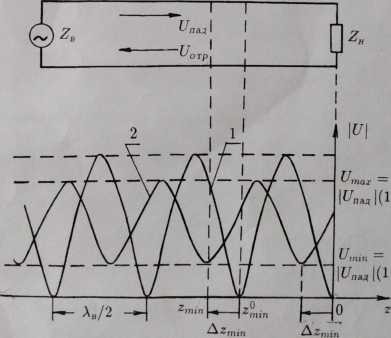
\includegraphics{img/2.jpg}
	\caption{Распределение модуля напряжения вдоль линии: 1 -- режим короткого замыкания ($Z_H=0$); 2 -- произвольный импеданс на конце линии ($Z_H\ne0$)}
	\label{fig:p1}
\end{figure}
В формуле (П.З)
\begin{equation}
	|\Gamma|=\left|\frac{U_\text{пад,H}}{U_\text{отр,H}}\right|=\left|\frac{U_\text{пад}}{U_\text{отр}}\right|,
\end{equation}
-- модуль коэффициента отражения, $\phi_H$ -- фаза коэффициента отражения в сечении нагрузки. Располагая начало координат $(z = 0)$ в плоскости нагрузки (рис. П.1), в произвольном сечении $z$ линии имеем
\begin{gather}
	U=U_\text{пад,H}e^{-ihz}+U_\text{отр,H}e^{ihz}=
		=U_\text{пад}(1+\Gamma e^{i2hz})=
		=U_\text{пад}(1+|\Gamma|e^{i\psi}),
\end{gather}
где
\begin{equation}
	\psi=\phi_H+2hz
\end{equation}
--- фаза коэффициента отражения в сечении 2, h -- постоянная распространения волны в линии.

Режим работы линии передачи удобно характеризовать коэффициентом стоячей волны К (КСВ), равным отношению максимального напряжения в линии к ее минимальному значению
\begin{equation}
	\mathrm { K } = \frac { | U | _ { \max } } { | U | _ { \min } }
\end{equation}
Иногда используется и обратная величина -- коэффициент бегущей волны (КБВ). В максимуме стоячей волны напряжения в падающей и отраженной волнах синфазны:
\begin{equation}
	|U|_{max}=|U_\text{пад}|+|U_\text{отр}|=|U_\text{пад}|(1+|\Gamma|),
\end{equation}
в минимуме -- противофазны:
\begin{equation}
	|U|_{min}=|U_\text{пад}|-|U_\text{отр}|=|U_\text{пад}|(1-|\Gamma|),
\end{equation}
Тогда
\begin{equation}
	\mathrm { K } = \frac { 1 + | \Gamma | } { 1 - | \Gamma | },
\end{equation}
откуда получим
\begin{equation}
	| \Gamma | = \frac { K - 1 } { K + 1 }
\end{equation}

Нетрудно убедиться в том, что К изменяется от единицы до бесконечности, причем режиму согласования, когда $Z_H = Z_B$, соответствует значение $\mathrm{К}=1$, а режиму короткого замыкания (или холостого хода), а также любой реактивной нагрузке -- $\mathrm{К}=\infty$.

Измерение К может быть произведено путем перемещения вдоль измерительной линии (ИЛ) прибора, показания которого связаны с высокочастотным напряжением в данном сечении линии. 
В случае коаксиальных и волноводных систем ИЛ снабжены зондом штыревого типа, расположенным вдоль силовых линий электрического поля и перемещающимся вдоль продольной щели. 
Схема ИЛ изображена на рис. П.2.
\begin{figure}[h!]
	\centering
	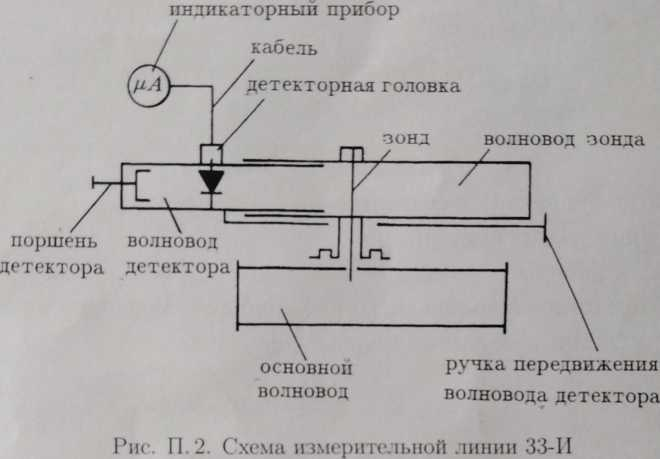
\includegraphics{img/3.jpg}
	\caption{Схема измерительной линии 33-И}
	\label{fig:figure1}
\end{figure}

Основной волновод измерительной линии включен в тракт испытуемой волноводной системы. 
При перемещении вдоль щели основного волновода зонд ответвляет часть электромагнитной энергии. 
Для детектирования СВЧ сигнала зонда в ИЛ обычно применяют кристаллические детекторы (СВЧ диоды). 
При этом зависимость между током детектора $I$ и приложенным высокочастотным напряжением $|U|$ является нелинейной.

Из теории детектирования известно, что при малых значениях переменного напряжения детектор имеет характеристику $I=f(|U|)$, близкую к квадратичной. В этом случае ток детектора
\begin{equation}
	I=\alpha|U|^2,
\end{equation}
где $\alpha$ --- параметр, зависящий от свойств детектора.

В максимуме и в минимуме распределения поля в линии имеем
\begin{equation}
	I _ { \max } = \alpha | U | _ { \min x } ^ { 2 } , \quad I _ { \min } = \alpha | U | _ { \min } ^ { 2 }
\end{equation}
откуда
\begin{equation}
	\mathrm { K } = \sqrt { \frac { I _ { \mathrm { max } } } { I _ { \mathrm { min } } } }
\end{equation}

Опыт показывает, что для современных стандартных кристаллических детекторов выражение (П.10) оказывается справедливым при выпрямленных токах менее $\sim20$ мкА.

Величину фазы коэффициента отражения в сечении $z$ ($z<0$) --- $\psi=\phi_H+2hz$ можно определить, например, зная положения точек $z_{min}$ минимального значения напряжения. Из (П.6) нетрудно видеть, что
\begin{equation}
	\psi \left( z _ { \min } \right) = ( 2 n - 1 ) \pi = \varphi _ { \mathrm { H } } + 2 h z _ { \min }
\end{equation}
и при $n = 0$ имеем

\begin{equation}
	\varphi _ { \mathrm { H } } = - 2 h z _ { \mathrm { min } } - \pi
\end{equation}

Таким образом, для определения фазы коэффициента отражения достаточно определить положение минимума напряжения в ИЛ\footnote{При характеристике детектора, близкой к квадратичной, минимум тока детектора никогда не бывает четко выраженным, особенно при небольших К. Для повышения точности отсчета положений минимумов $z_{\min}$ применяют метод <<вилки>>, состоящий в определении двух положений зонда $z_1$ и $z_2$ при одинаковых показаниях индикатора и вычислении $z_{\min}$ по формуле $z_{\min}=(z_1+z_2)/2$.} относительно плоскости присоединения нагрузки. 
%
Для этого необходимо найти т.н. \textbf{условный конец линии} -- сечение волновода, соответствующее минимуму напряжения при коротком замыкании линии ($z^0_{min}$ на рис. П.1), и заменить в (П.13) величину $Z_{min}$ на $(z_{min}-z_{min}^0)$. 
Расстояние от условного конца линии $z^0_{min}$ до ближайшего минимума напряжения $z_{min}$ \textbf{со стороны генератора} при включенной нагрузке обозначим через 
$\Delta z _ { \min } \equiv z _ { \min } ^ { 0 } - z _ { \min } = \left| z _ { \min } - z _ { \min } ^ { 0 } \right| =- \left( z _ { \min } - z _ { \min } ^ { 0 } \right)$

Тогда, согласно (П.13),  $\varphi _ { \mathrm { H } } = 2 h \Delta z _ { \mathrm { min } } - \pi$ и фаза коэффициента отражения (с учетом выражения $h=2\pi/\lambda_B$) будет определяться формулой
\begin{equation}
	\varphi _ { \mathrm { H } } = 4 \pi \frac { \Delta z _ { \mathrm { min } } } { \lambda _ { \mathrm { B } } } - \pi
\end{equation}

\end{document}